\documentclass[tikz,border=3pt]{standalone}
\usepackage[T1]{fontenc}
\usepackage{lmodern,amsmath}
\usetikzlibrary{arrows.meta,calc,patterns}
\begin{document}
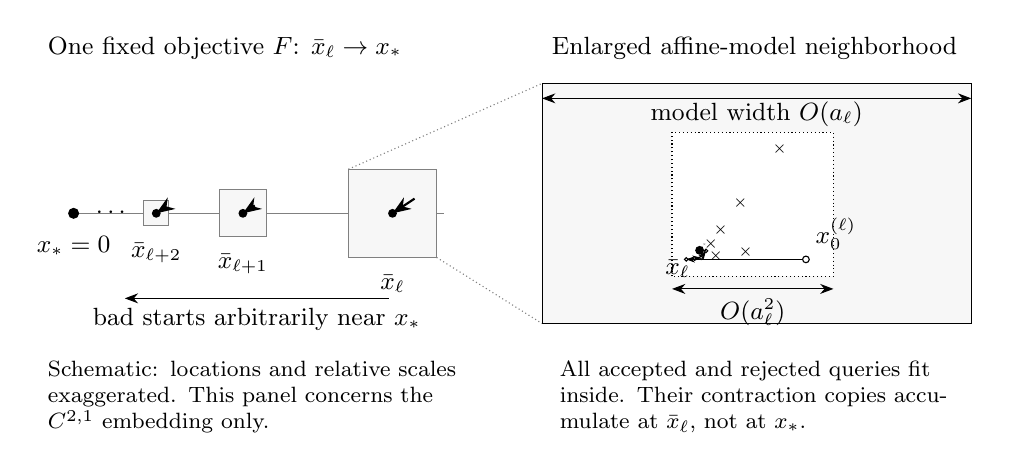
\begin{tikzpicture}[>=Stealth,font=\small,
phase0/.style={solid},phase1/.style={densely dashed},
phase2/.style={dash pattern=on 4pt off 1.6pt on .7pt off 1.6pt}]
\node[anchor=west] at (0,3.6) {One fixed objective $F$: $\bar x_\ell\to x_*$};
\node[anchor=west] at (6.4,3.6) {Enlarged affine-model neighborhood};
\draw[gray] (.45,1.5)--(5.15,1.5);
\fill (.45,1.5) circle[radius=2pt] node[below=5pt] {$x_*=0$};
\node at (.95,1.5) {$\cdots$};
\draw[gray,fill=black!3] (1.340000000,1.340000000) rectangle (1.660000000,1.660000000);
\fill (1.500000000,1.500000000) circle[radius=1.6pt];
\node[below] at (1.500000000,1.240000000) {$\bar x_{\ell+2}$};
\draw[->,thick] (1.580000000,1.553333333)--(1.500000000,1.500000000);
\draw[gray,fill=black!3] (2.300000000,1.200000000) rectangle (2.900000000,1.800000000);
\fill (2.600000000,1.500000000) circle[radius=1.6pt];
\node[below] at (2.600000000,1.100000000) {$\bar x_{\ell+1}$};
\draw[->,thick] (2.750000000,1.600000000)--(2.600000000,1.500000000);
\draw[gray,fill=black!3] (3.940000000,0.940000000) rectangle (5.060000000,2.060000000);
\fill (4.500000000,1.500000000) circle[radius=1.6pt];
\node[below] at (4.500000000,0.840000000) {$\bar x_{\ell}$};
\draw[->,thick] (4.780000000,1.686666667)--(4.500000000,1.500000000);
\draw[->] (4.45,.42)--(1.10,.42) node[midway,below] {bad starts arbitrarily near $x_*$};
\draw[densely dotted,gray] (3.94,2.06)--(6.4,3.15);
\draw[densely dotted,gray] (5.06,.94)--(6.4,.1);
\draw[fill=black!3] (6.4,.1) rectangle (11.85,3.15);
\draw[<->] (6.4,2.96)--(11.85,2.96) node[midway,below,inner sep=1pt] {model width $O(a_\ell)$};
\draw[fill=white,densely dotted] (8.05,.70) rectangle (10.1,2.53);
\begin{scope}[shift={(8.40cm,1.03cm)},x=1.52cm,y=1.40cm]
\draw[->,>={Stealth[length=1.1mm,width=.8mm]},phase0,line width=.35pt] (0.888432624,-0.082297398)--(-0.111567376,-0.082297398);
\draw[->,>={Stealth[length=1.1mm,width=.8mm]},phase1,line width=.35pt] (-0.111567376,-0.082297398)--(0.012456062,-0.066672398);
\draw[->,>={Stealth[length=1.1mm,width=.8mm]},phase2,line width=.35pt] (0.012456062,-0.066672398)--(0.053482939,-0.004954238);
\draw[fill=white] (-0.111567376,-0.082297398) circle[radius=.65pt];
\node[inner sep=0pt,font=\tiny,scale=1.000000] at (0.384526374,-0.019797398) {$\times$};
\node[inner sep=0pt,font=\tiny,scale=1.000000] at (0.136479499,-0.051047398) {$\times$};
\draw[fill=white] (0.012456062,-0.066672398) circle[radius=.65pt];
\node[inner sep=0pt,font=\tiny,scale=1.000000] at (0.668886094,0.920818157) {$\times$};
\node[inner sep=0pt,font=\tiny,scale=1.000000] at (0.340671078,0.427072880) {$\times$};
\node[inner sep=0pt,font=\tiny,scale=1.000000] at (0.176563570,0.180200241) {$\times$};
\node[inner sep=0pt,font=\tiny,scale=1.000000] at (0.094509816,0.056763922) {$\times$};
\draw[fill=white] (0.053482939,-0.004954238) circle[radius=.65pt];
\draw[phase0,line width=.35pt] (0.053482939,-0.004954238)--(-0.006716267,-0.004954238);
\draw[phase1,line width=.35pt] (-0.006716267,-0.004954238)--(0.000749845,-0.004013625);
\draw[phase2,line width=.35pt] (0.000749845,-0.004013625)--(0.003219630,-0.000298241);
\draw[fill=white] (-0.006716267,-0.004954238) circle[radius=.25pt];
\node[inner sep=0pt,font=\tiny,scale=0.245355] at (0.023148182,-0.001191788) {$\times$};
\node[inner sep=0pt,font=\tiny,scale=0.245355] at (0.008215957,-0.003073013) {$\times$};
\draw[fill=white] (0.000749845,-0.004013625) circle[radius=.25pt];
\node[inner sep=0pt,font=\tiny,scale=0.245355] at (0.040266412,0.055432522) {$\times$};
\node[inner sep=0pt,font=\tiny,scale=0.245355] at (0.020508128,0.025709448) {$\times$};
\node[inner sep=0pt,font=\tiny,scale=0.245355] at (0.010628987,0.010847911) {$\times$};
\node[inner sep=0pt,font=\tiny,scale=0.245355] at (0.005689416,0.003417143) {$\times$};
\draw[fill=white] (0.003219630,-0.000298241) circle[radius=.25pt];
\draw[phase0,line width=.35pt] (0.003219630,-0.000298241)--(-0.000404314,-0.000298241);
\draw[phase1,line width=.35pt] (-0.000404314,-0.000298241)--(0.000045140,-0.000241617);
\draw[phase2,line width=.35pt] (0.000045140,-0.000241617)--(0.000193819,-0.000017954);
\draw[fill=white] (-0.000404314,-0.000298241) circle[radius=.25pt];
\node[inner sep=0pt,font=\tiny,scale=0.060199] at (0.001393502,-0.000071745) {$\times$};
\node[inner sep=0pt,font=\tiny,scale=0.060199] at (0.000494594,-0.000184993) {$\times$};
\draw[fill=white] (0.000045140,-0.000241617) circle[radius=.25pt];
\node[inner sep=0pt,font=\tiny,scale=0.060199] at (0.002424006,0.003336994) {$\times$};
\node[inner sep=0pt,font=\tiny,scale=0.060199] at (0.001234573,0.001547688) {$\times$};
\node[inner sep=0pt,font=\tiny,scale=0.060199] at (0.000639857,0.000653036) {$\times$};
\node[inner sep=0pt,font=\tiny,scale=0.060199] at (0.000342498,0.000205709) {$\times$};
\draw[fill=white] (0.000193819,-0.000017954) circle[radius=.25pt];
\fill (0,0) circle[radius=1.6pt];
\node[below left] at (0,0) {$\bar x_\ell$};
\draw[fill=white] (0.888432624,-0.082297398) circle[radius=1.2pt] node[above right] {$x_0^{(\ell)}$};
\end{scope}
\draw[<->] (8.05,.54)--(10.1,.54) node[midway,below] {$O(a_\ell^2)$};
\node[anchor=north west,align=left,text width=5.3cm,font=\footnotesize] at (6.5,-.25) {All accepted and rejected queries fit inside. Their contraction copies accumulate at $\bar x_\ell$, not at $x_*$.};
\node[anchor=north west,font=\footnotesize,align=left,text width=5.3cm] at (0,-.25) {Schematic: locations and relative scales exaggerated. This panel concerns the $C^{2,1}$ embedding only.};
\end{tikzpicture}
\end{document}
